\documentclass{article}
\usepackage[utf8]{inputenc}
\usepackage[a4paper, total={6.5in, 9in}]{geometry}
\usepackage{fancyhdr}
\usepackage{amsmath, amsthm, amsfonts, mathrsfs}
\usepackage{xcolor}
\usepackage{mathtools, float, subfig}
\renewcommand{\labelenumii}{(\roman{enumii})}

\newcommand{\rr}{\mathscr{R}_0}

\setlength{\headsep}{4em}
\pagestyle{fancy}
\setlength{\parindent}{0cm}
\setlength{\parskip}{1em}

% ASSIGNMENT INFORMATION
\newcommand{\class}{MATH 490}
\newcommand{\hwnumber}{5}

\lhead{Braden Hoagland (bch29)}
\chead{{\class} - HW {\hwnumber}}
\rhead{\today}

\begin{document}
\begin{enumerate}
	\item 
	\begin{enumerate}
		\item Let $X$ denote the number of days that an infected person remains infected. Then $X$ is distributed geometrically, i.e. $ \mathbb{P}(X=k) = \sigma^{i-1} (1-\sigma)$. Then the expected infection length is \[ \mathbb{E}[X] = \sum_{k=1}^{\infty} \sigma^{k-1}=\sum_{k=0}^{\infty} \sigma^{k}= \frac{1}{1-\sigma} .\]

		\item When $I_{t,j} \approx 0$, then
			\begin{align*}
				S_{t+1,j}&=S_{t,j}G_{t,j}\\
					 &= S_{t,j}e^{-\sum_{k=1}^{m} \beta_{j,k}I_{t,k}} \\
					 &\approx S_{t,j}e^{\sum_{k=1}^{m} \beta_{j,k} \cdot 0} \\
					 &= S_{t,j}
			\end{align*}
			Similarly, we can show $S_{t,j}\approx S_{t-1,j}$. Continuing, we get $S_{t,j}\approx S_{0,j}$.

			Now we take the Taylor expansion $e^x = 1 + x + \mathcal{O}(x^2)$ to show $e^x \approx 1 + x$ when $x$ is small. In the context of this problem, since $I_{t,j}$ is small, this means $e^{-\sum_k \beta_{j,k} I_{t,k}} \approx -\sum_{k} \beta_{j,k}I_{t,k} $. We can use this approximation, along with the approximation of $S$, to get
			\begin{align*}
				I_{t+1,j}&=S_{t,j}(1-G_{t,j}) + \sigma I_{t,j} \\
					 &\approx \sigma I_{t,j} + S_{0,j} \sum_{k=1}^{m} \beta_{j,k}I_{t,k} \\
					 &= \sigma I_{t,j} + \sum_{k=1}^{m} A_{j,k}I_{t,k}
			\end{align*}
			We can interpret $A_{j,k}$ as the rate of infectious contact between infectious type $k$'s and susceptible type $j$'s in a fully susceptible population.

		\item If we define $A_{j,k} = \eta_j \beta_{j,k}$, then the system of infected individuals can be written in vector form as $I_{t+1} = (\sigma+A) I_t$, the same as in the previous problem. We can then reasonably define $\rr(\eta)$ to be the maximum eigenvalue of $\sigma+A$. Such an $\rr(\eta)$ would then quantify the largest increase to a component (type) of $I_{t}$.

		\item In this example, $A$ is
			\[
			A=
			\begin{pmatrix}
				0.47 p & 0.08 p \\
				0.93(1-p) & 1.2(1-p)
			\end{pmatrix}
			\] 
			and the matrix $\sigma + A$ is
			\[
			\sigma+A=
			\begin{pmatrix}
				0.75+0.47p & 0.75+0.08p \\
				1.68-0.93p & 1.95-1.2p
			\end{pmatrix}.
			\] 
			Both eigenvalues of $\sigma+A$ as a function of $p\in[0,1]$ are plotted below. Since we defined $\rr(\eta)$ to be the maximum eigenvalue, $\rr(\eta)$ is shown by the line labeled $\lambda_+$.

			\begin{figure}[H]
				\centering
				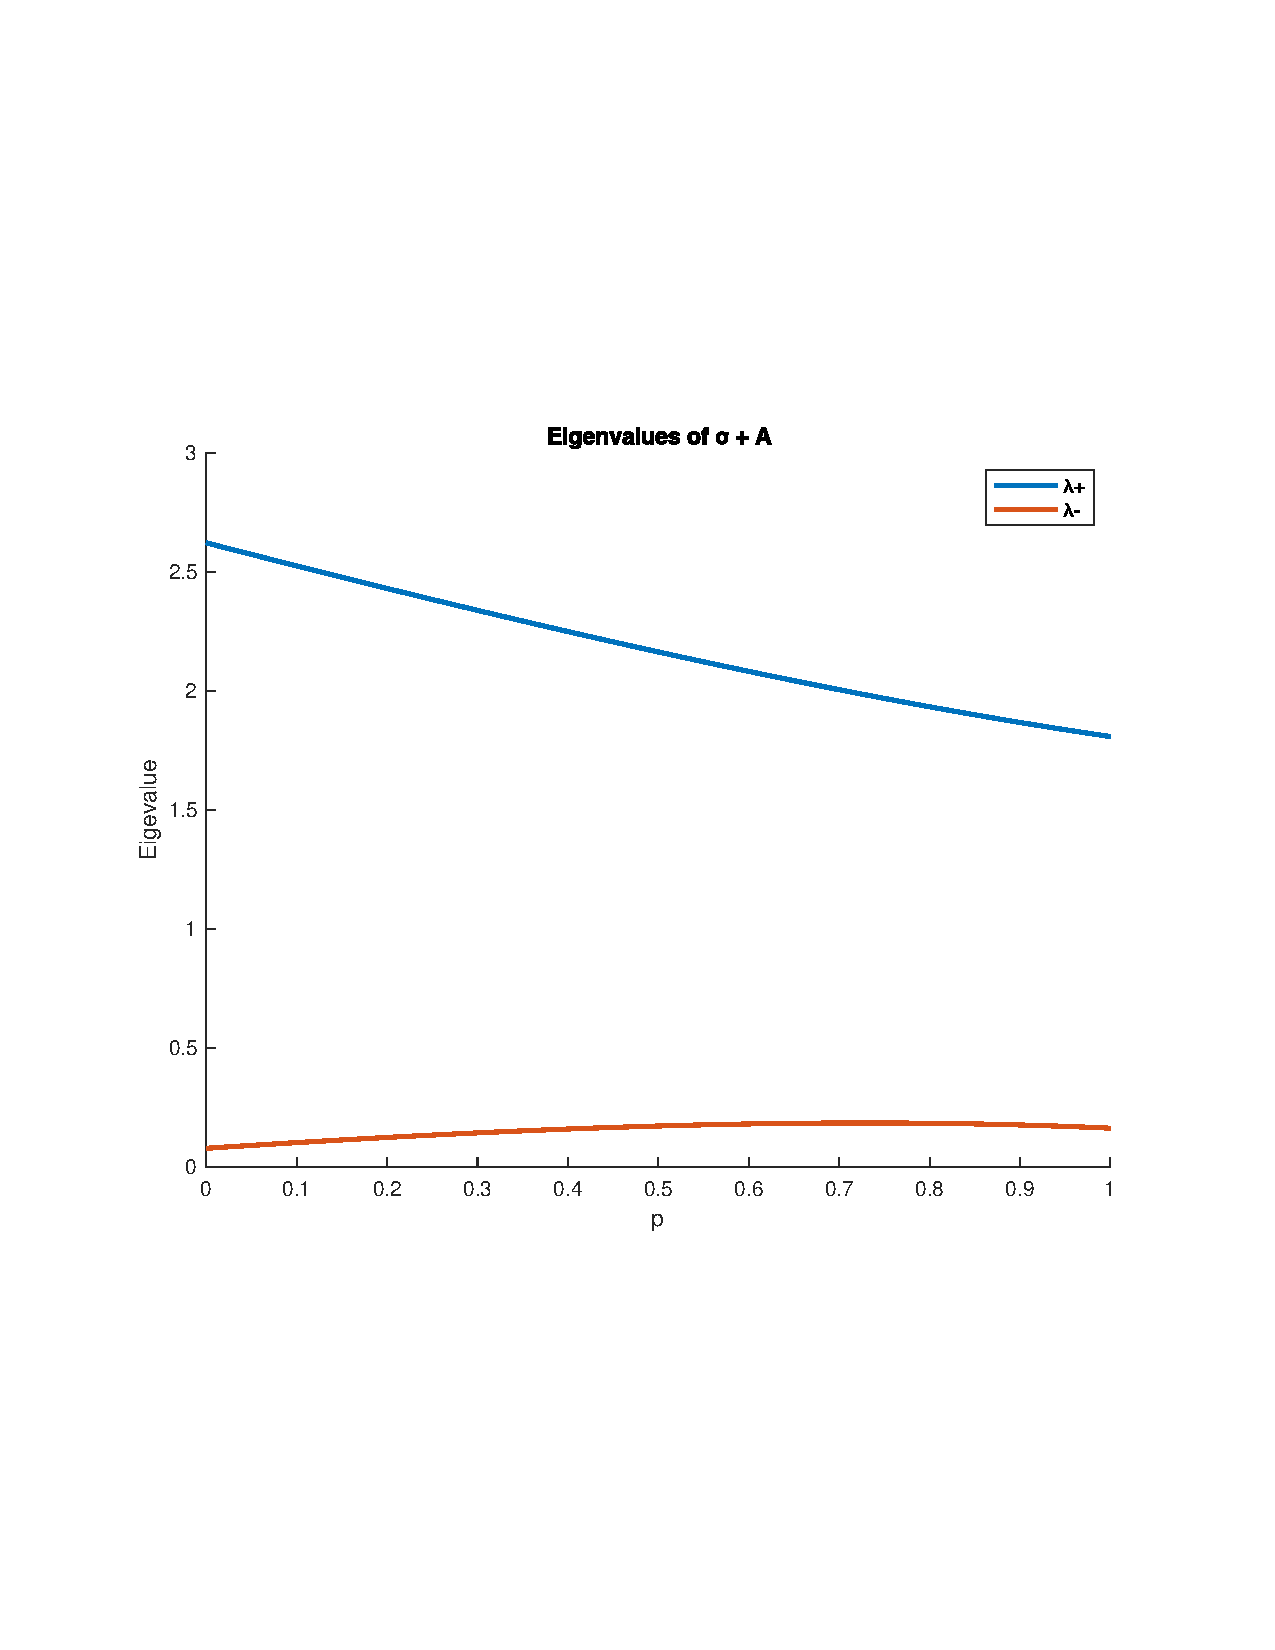
\includegraphics[scale=0.4]{img/eigs.pdf}
			\end{figure}

		\item 
			Solving the model numerically for 60 timesteps yields the following.
			\begin{figure}[H]
				\centering
				\subfloat{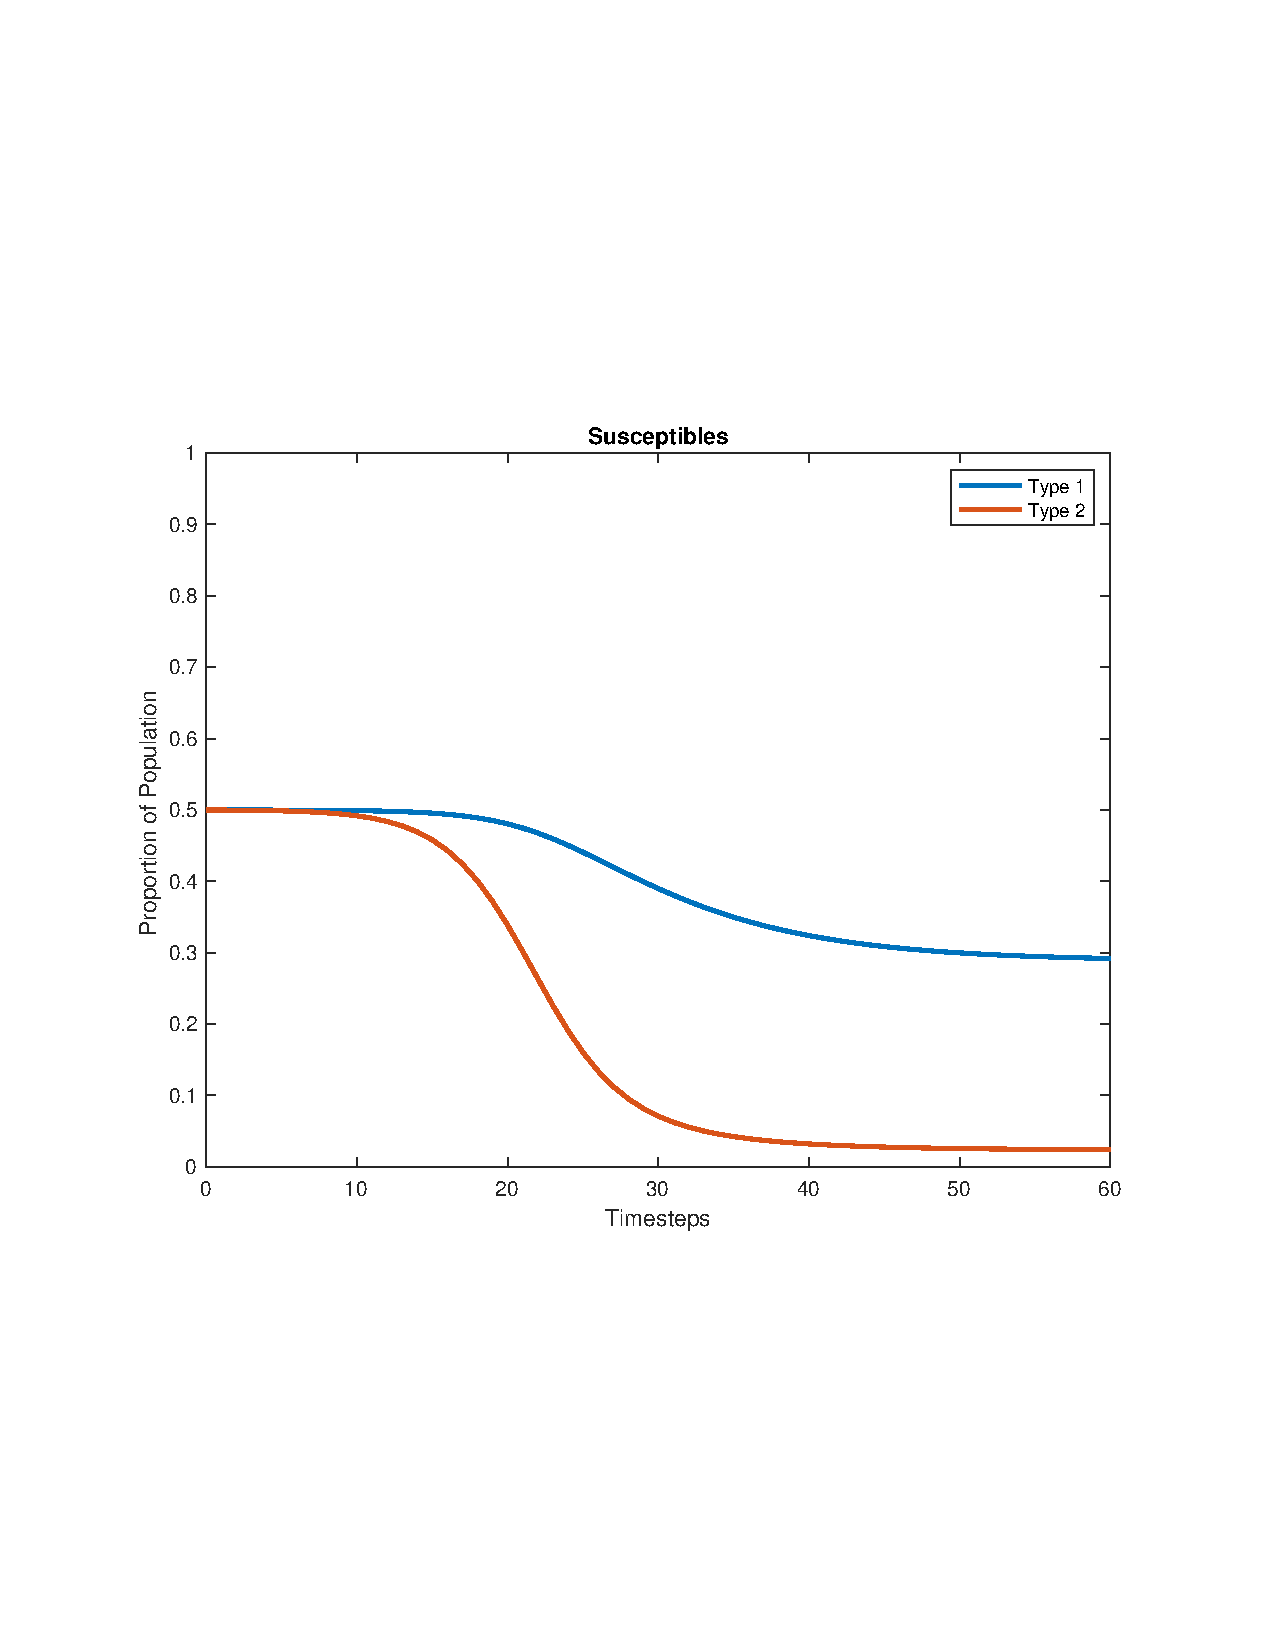
\includegraphics[scale=0.35]{img/S.pdf}}
				\subfloat{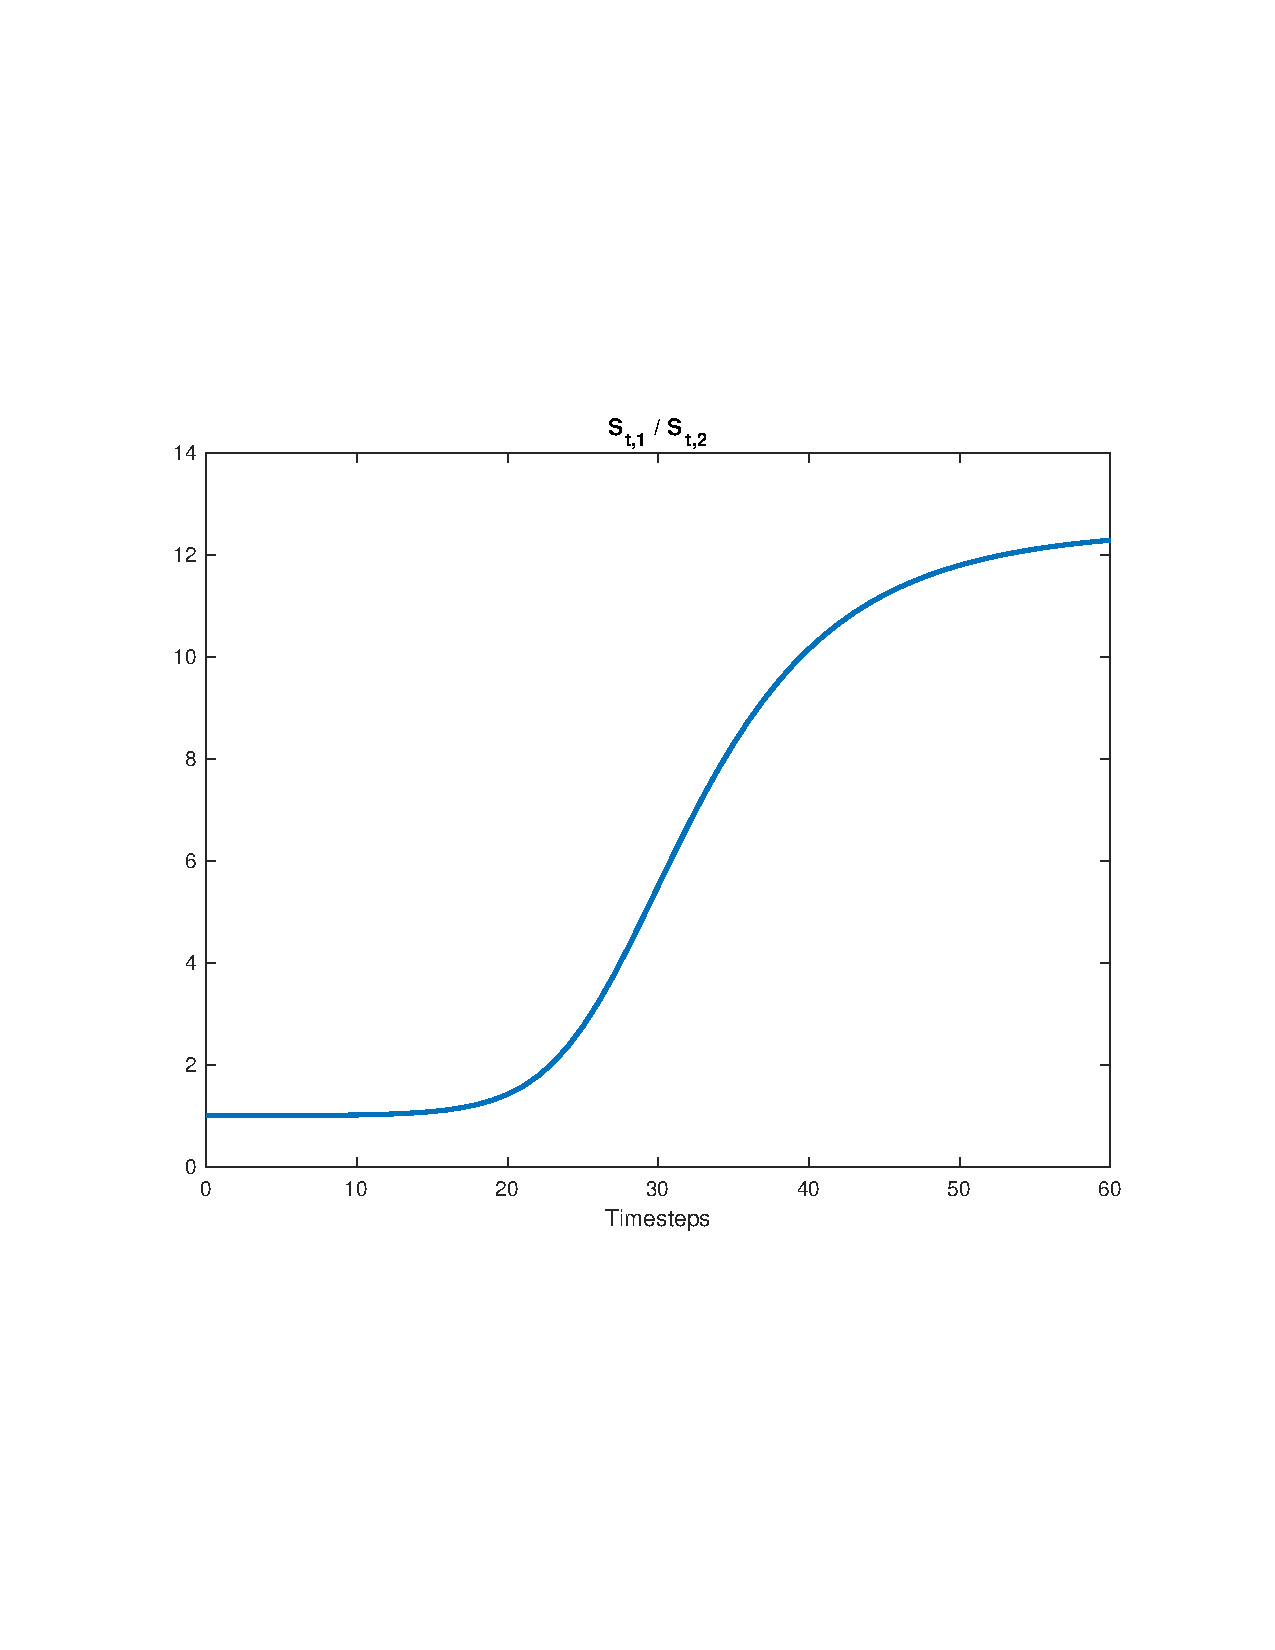
\includegraphics[scale=0.35]{img/ratio.pdf}}
			\end{figure}
			From the first figure we can see that the total number of susceptibles is decreasing, and from the second figure we can see that the number of type 1 susceptibles is growing relative to the number of type 2 susceptibles.
			We can evaluate the matrix $A$ given $\eta = (1/2, 1/2)$ to get
			\[
			A=
			\begin{pmatrix}
				0.235 & 0.04 \\
				0.465 & 0.6
			\end{pmatrix}
			\] 
	Since we interpreted $A_{j,k}$ as the rate of infectious contact between infectious type $k$'s and susceptible type $j$'s in a fully susceptible population, the sum of row $j$ in $A$ can be interpreted as the total rate of infectious contact with susceptible type $j$'s. From this it is clear that substantially less infectious contact is being made with type 1 than type 2, which explains why fewer type 1's contract the disease in the simulated model.
	\end{enumerate}
\end{enumerate}
\end{document}
